\documentclass[12pt, journal, onecolumn]{IEEEtran}
\usepackage{colortbl}
\usepackage{booktabs}
\usepackage{subcaption}
\usepackage{algorithm}
\usepackage{algorithmicx}
\usepackage{algpseudocode}
\usepackage{tabulary}
\usepackage{bigstrut}
\setlength\fboxsep{1pt}
\setlength\fboxrule{1pt}
\usepackage{multicol}
%\bstctlcite{IEEEexample:BSTcontrol}
\usepackage[table]{xcolor}
\usepackage{picture}
\newcommand{\quart}[4]{\begin{picture}(100,3)
  {\color{black}\put(#3,3){\circle*{4}}\put(#1,3){\line(1,0){#2}}}\end{picture}}
\usepackage{amsmath}
\usepackage{balance}
\usepackage{flushend}
\usepackage[english]{babel}
\usepackage{blindtext}
\usepackage{times}
\usepackage{cite}
\usepackage{graphicx}
\usepackage{hyperref}
\hypersetup{
  colorlinks = false,
  hidelinks = true
}
\setlength{\parindent}{0em}
\setlength{\parskip}{1em}

\begin{document}
  \title{Research Study Project Submittal Preparation}
%  \author{Rahul Krishna, 
%    \IEEEauthorblockA{\normalsize {\textit{Dept. of Electrical and Computer 
%          Engineering}\\
%        North Carolina State University, Email: 
%        \href{mailto:rkrish11@ncsu.edu}{{rkrish11@ncsu.edu}}}}}
  
    \maketitle
    \section{Project description and References (1 Point)}
      \noindent Programming inherently introduces defects into programs, as a result software systems can crash or fail to deliver an important functionality. It is very important to test a software throughly before it can be used. But an extensive testing can be prohibitively expensive or may take too much time to conduct This necessitates the use of automated software defect prediction tools. Although numerous machine learning algorithms are available to detect defects in software, several factors undermine the accuracy of such algorithm. 
      
      This paper uses Classification and Regression Trees (CART) and Random Forests to examines two approaches to counter the aforementioned problem. The first approach involves the use Synthetic Minority Oversampling Technique (also known as SMOTE). The second approach attempts to use a metaheursitic algorithm such as differential evolution to find the right set of parameters that can change the performance of the predictor.
 
\begin{thebibliography}{10}
\bibitem{smote1}
Chawla, N. V., Bowyer, K. W., Hall, L. O., \& Kegelmeyer, W. P. (2002). SMOTE: synthetic minority over-sampling technique. Journal of artificial intelligence research, 16(1), 321-357.
\bibitem{smote2}
Pelayo, L.; Dick, S., "Applying Novel Resampling Strategies To Software Defect Prediction," Fuzzy Information Processing Society, 2007. NAFIPS '07. Annual Meeting of the North American , June 2007.
\bibitem{tunelearners}
Fu, W., \& Menzies, T. ``Analytics Without Parameter Tuning Considered Harmful?'', Unpublished manuscript, North Carolina State University, Raleigh NC.
\bibitem{prec}
Menzies, Tim, et al. "Problems with precision: A response to “comments on ‘data mining static code attributes to learn defect predictors’”." IEEE Transactions on Software Engineering 33.9 (2007): 637.
\bibitem{defect1}
E. Barr P. Devanbu F. Rahman, S. Khatri. Comparing static bug finders and
statistical prediction. ICSE’14, 2014.
\bibitem{openscience}
Tim Menzies, Carter Pape, Mitch Rees-Jones, and Rahul Krishna. The promise repository of empirical software engineering data, Feb 2015.
\bibitem{scottknott}
Scott, A. J., \& Knott, M. (1974). A cluster analysis method for grouping means in the analysis of variance. Biometrics, 507-512.
\end{thebibliography}
\newpage
\section{Models and Equations (2 Points)}
The proposed techniques do not use any explicit models or equations. I am therefore including a sample tree generated by CART (see \ref{fig:CARTtree}) and the pseudocode of the Differential Evolution algorithm \ref{alg:DE}
\begin{figure}[h!]
  \centering
  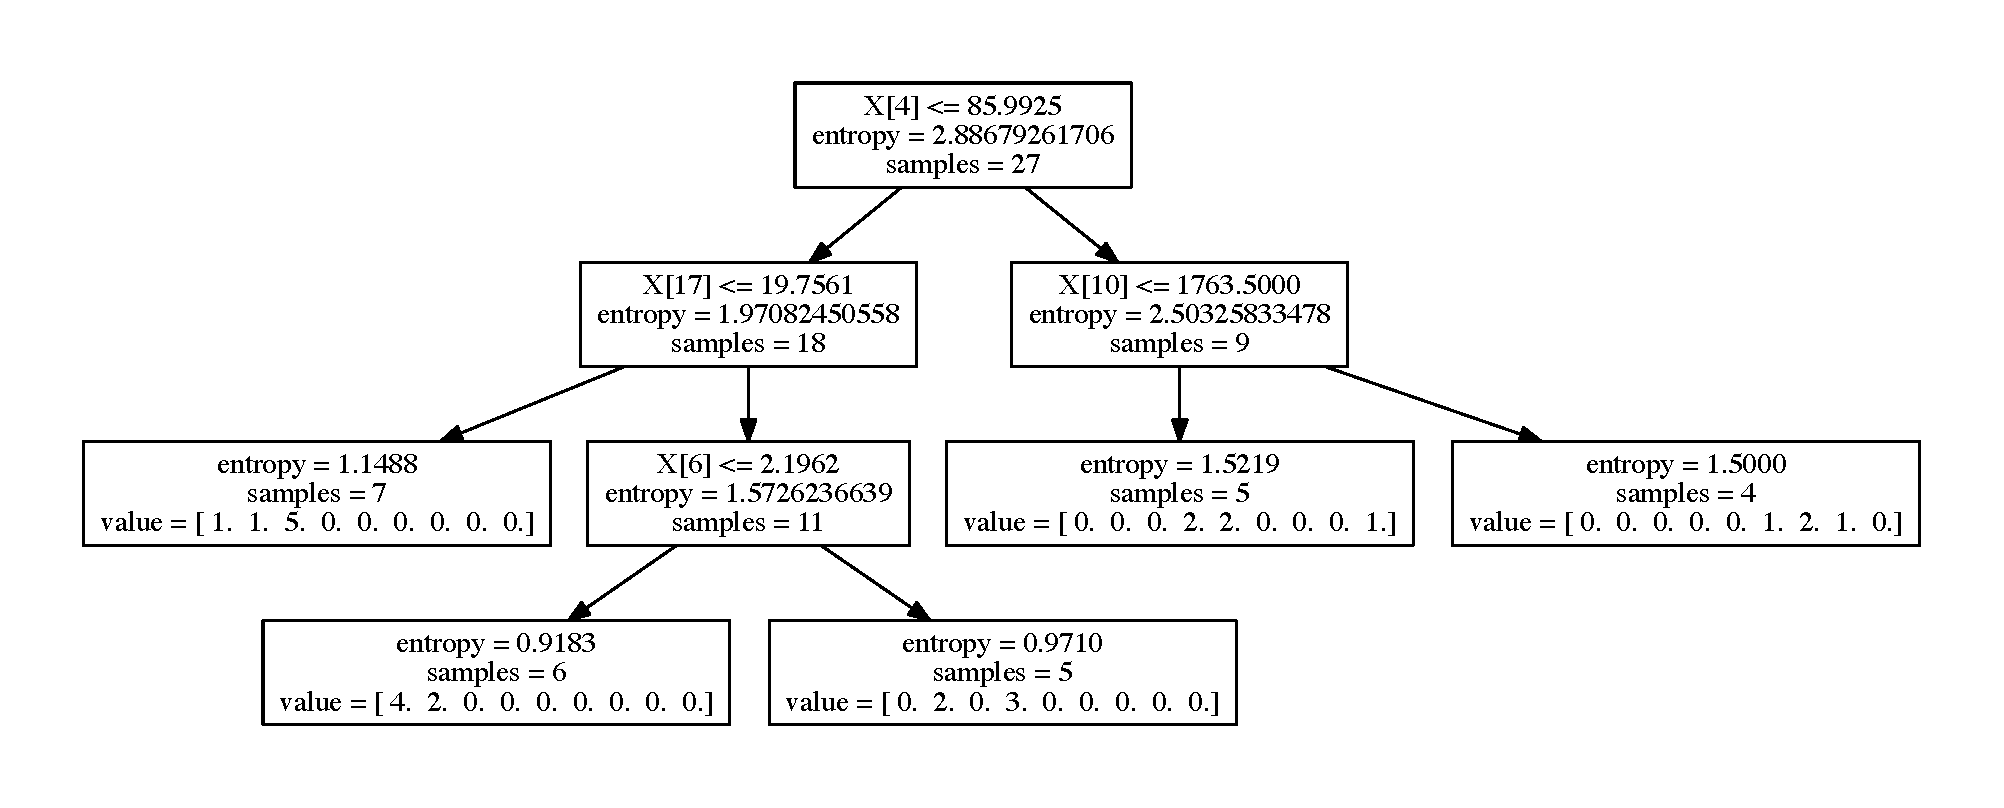
\includegraphics[width=0.9\linewidth]{tree2.pdf}
  \caption{CART Tree example} \label{fig:CARTtree}
\end{figure}
\begin{figure}[h!]
  \centering
  \begin{minipage}{0.5\linewidth}
  \renewcommand{\baselinestretch}{0.8}\begin{center}\scriptsize
  \begin{algorithmic}[1]
    \Require $\mathit{np} = 10$, $f=0.75$, $cr=0.3$, $\mathit{life} = 5$, $\mathit{Goal} \in \{\mathit{pd},f,...\}$
    \Ensure $S_{best}$
    
    ~\\
    \Function{DE}{$\mathit{np}$, $f$, $cr$, $\mathit{life}$, $\mathit{Goal}$}
    \State $Population  \gets $ $InitializePopulation$($\mathit{np}$)   
    \State $S_{best} \gets $$GetBestSolution$($Population $)
    \While{$\mathit{life} > 0$}
    \State $NewGeneration \gets \emptyset$
    \For{$i=0 \to \mathit{np}-1$}
    \State $S_i \gets$ Extrapolate($Population [i], Population , cr, f$)
    \If {Score($S_i$)$\ge$Score($Population [i]$)}
    \State $NewGeneration$.$append$($S_i$)
    \Else
    \State $NewGeneration$.$append$($Population [i]$)
    \EndIf
    \EndFor
    \State $Population  \gets NewGeneration$
    \If{$\neg$ $Improve$($Population $)}
    \State $life -=1$
    \EndIf
    \State $S_{best} \gets$ $GetBestSolution$($Population $)
    \EndWhile
    \State \Return $S_{best}$
    \EndFunction
    \Function{Score}{$Candidate$}
    \State set tuned parameters according to $Candidate$
    \State $model \gets$$TrainLearner()$
    \State $result \gets$$TestLearner$($model$)   
    \State \Return$\mathit{Goal}(result)$  
    \EndFunction
    \Function{Extrapolate}{$old, pop, cr, f$}
    \State $a, b, c\gets threeOthers(pop,old)$  
    \State $newf \gets \emptyset$
    \For{$i=0 \to \mathit{np}-1$}
    \If{$cr < random()$}
    \State $newf$.$append$($old[i]$)
    \Else
    \If{typeof($old[i]$) == bool}
    \State $newf$.$append$(not $old[i]$)
    \Else
    \State $newf$.$append$(trim($i$,($a[i] + f * (b[i] - c[i]$)))) 
    \EndIf
    \EndIf
    \EndFor
    \State \Return $newf$
    \EndFunction
  \end{algorithmic} 
  \caption{Pesudocode for DE with Early Termination}
  \label{alg:DE}
\end{center}
\end{minipage}
\end{figure}

\section{Metrics, graphs tables and charts (1 Point)}
Figure \ref{fig:ck} lists all the metrics used by the datasets. Figure \ref{fig:sk} contains the preliminary results of my tests.
\begin{figure}[h]
  \renewcommand{\baselinestretch}{0.9}\begin{center}
    {\scriptsize
      \begin{tabular}{c|l|p{4.7in}}
        amc & average method complexity & e.g. number of JAVA byte codes\\\hline
        avg\_cc & average McCabe & average McCabe's cyclomatic complexity seen
        in class\\\hline
        ca & afferent couplings & how many other classes use the specific
        class. \\\hline
        cam & cohesion amongst classes & summation of number of different
        types of method parameters in every method divided by a multiplication
        of number of different method parameter types in whole class and
        number of methods. \\\hline
        cbm &coupling between methods &  total number of new/redefined methods
        to which all the inherited methods are coupled\\\hline
        cbo & coupling between objects & increased when the methods of one
        class access services of another.\\\hline
        ce & efferent couplings & how many other classes is used by the
        specific class. \\\hline
        dam & data access & ratio of the number of private (protected)
        attributes to the total number of attributes\\\hline
        dit & depth of inheritance tree &\\\hline
        ic & inheritance coupling &  number of parent classes to which a given
        class is coupled (includes counts of methods and variables inherited)
        \\\hline
        lcom & lack of cohesion in methods &number of pairs of methods that do
        not share a reference to an instance variable.\\\hline
        locm3 & another lack of cohesion measure & if $m,a$ are  the number of
        $methods,attributes$
        in a class number and $\mu(a)$  is the number of methods accessing an
        attribute, 
        then
        $lcom3=((\frac{1}{a} \sum_j^a \mu(a_j)) - m)/ (1-m)$.
        \\\hline
        loc & lines of code &\\\hline
        max\_cc & maximum McCabe & maximum McCabe's cyclomatic complexity seen
        in class\\\hline
        mfa & functional abstraction & number of methods inherited by a class
        plus number of methods accessible by member methods of the
        class\\\hline
        moa &  aggregation &  count of the number of data declarations (class
        fields) whose types are user defined classes\\\hline
        noc &  number of children &\\\hline
        npm & number of public methods & \\\hline
        rfc & response for a class &number of  methods invoked in response to
        a message to the object.\\\hline
        wmc & weighted methods per class &\\\hline
        \rowcolor{lightgray}
        defect & defect & Boolean: where defects found in post-release bug-tracking systems.
        \end{tabular}
        }
\end{center}
\caption{OO measures used in our defect data sets.  Last line is
the dependent attribute (whether a defect is reported to  a
post-release bug-tracking system).}\label{fig:ck}
\end{figure}
\begin{figure}[h!]
  \renewcommand{\baselinestretch}{1.1}
\begin{subtable}{0.5\linewidth}

{\tiny \begin{tabulary}{\linewidth}{|J|J|J|J|J|}
\hline
\textbf{Rank} & \textbf{Treatment} & \textbf{Med} & \textbf{IQR} & \textbf{Quartiles}\\\hline
1 &   RF &    41.0  &  3.0 & \quart{0}{7}{2}{-102} \\
\hline  2 &   CART &    44.0  &  3.0 & \quart{10}{8}{10}{-102} \\
\hline  3 & CART (SMOTE) &    70.0  &  2.0 & \quart{76}{5}{78}{-102} \\
\hline  4 & RF (SMOTE) &    78.0  &  1.0 & \quart{97}{2}{99}{-102} \\
\hline \end{tabulary}} \caption{ant} \label{ant}

\end{subtable}
\begin{subtable}{0.5\linewidth}
{\tiny \begin{tabulary}{\linewidth}{|J|J|J|J|J|}
\hline
\textbf{Rank} & \textbf{Treatment} & \textbf{Med} & \textbf{IQR} & \textbf{Quartiles}\\\hline
1 & RF &    39.0  &  1.0 & \quart{0}{4}{0}{-172} \\
\hline  2 & CART &    43.0  &  2.0 & \quart{9}{9}{18}{-172} \\
\hline  3 & CART (SMOTE) &    56.0  &  2.0 & \quart{72}{9}{77}{-172} \\
\hline  4 & RF (SMOTE) &    60.0  &  2.0 & \quart{90}{9}{95}{-172} \\
\hline \end{tabulary}}\caption{Camel} \label{Camel}

\end{subtable}\\[0.2cm]

\begin{subtable}{0.5\linewidth}
{\tiny \begin{tabulary}{\linewidth}{|J|J|J|J|J|}
\hline
\textbf{Rank} & \textbf{Treatment} & \textbf{Med} & \textbf{IQR} & \textbf{Quartiles}\\\hline
1 & RF (SMOTE) &    0.0  &  0.0 & \quart{0}{0}{0}{1} \\
1 & CART (SMOTE) &    15.0  &  15.0 & \quart{0}{26}{26}{1} \\
\hline  2 &   RF &    50.0  &  1.0 & \quart{85}{2}{87}{1} \\
\hline  3 &   CART &    56.0  &  1.0 & \quart{98}{1}{98}{1} \\
\hline \end{tabulary}}\caption{Ivy} \label{Camel}

\end{subtable}
\begin{subtable}{0.5\linewidth}
{\tiny \begin{tabulary}{\linewidth}{|J|J|J|J|J|}
\hline
\textbf{Rank} & \textbf{Treatment} & \textbf{Med} & \textbf{IQR} & \textbf{Quartiles}\\\hline
1 & RF &    0.0  &  0.0 & \quart{0}{0}{0}{1} \\
1 & CART (SMOTE) &    84.0  &  1.0 & \quart{89}{1}{90}{1} \\
1 & RF (SMOTE) &    88.0  &  1.0 & \quart{93}{1}{94}{1} \\
1 & CART &    93.0  &  0.0 & \quart{99}{0}{99}{1} \\
\hline \end{tabulary}}\caption{Jedit} \label{Camel}

\end{subtable}\\[0.2cm]

\begin{subtable}{0.5\linewidth}
{\tiny \begin{tabulary}{\linewidth}{|J|J|J|J|J|}
\hline
\textbf{Rank} & \textbf{Treatment} & \textbf{Med} & \textbf{IQR} & \textbf{Quartiles}\\\hline
1 &   CART &    36.0  &  3.0 & \quart{0}{14}{0}{-166} \\
1 &   RF &    40.0  &  4.0 & \quart{4}{19}{19}{-166} \\
\hline  2 & RF (SMOTE) &    53.0  &  6.0 & \quart{71}{28}{80}{-166} \\
2 & CART (SMOTE) &    54.0  &  4.0 & \quart{76}{19}{85}{-166} \\
\hline \end{tabulary}}\caption{POI} \label{Camel}

\end{subtable}
\begin{subtable}{0.5\linewidth}
{\tiny \begin{tabulary}{\linewidth}{|J|J|J|J|J|}
\hline
\textbf{Rank} & \textbf{Treatment} & \textbf{Med} & \textbf{IQR} & \textbf{Quartiles}\\\hline
1 & RF (SMOTE) &    2.0  &  2.0 & \quart{0}{4}{2}{0} \\
\hline  2 & CART (SMOTE) &    14.0  &  5.0 & \quart{31}{12}{31}{0} \\
\hline  3 & RF &    22.0  &  2.0 & \quart{48}{5}{51}{0} \\
\hline  4 & CART &    41.0  &  2.0 & \quart{95}{4}{97}{0} \\
\hline \end{tabulary}}\caption{Log4j} \label{Camel}

\end{subtable}\\[0.2cm]

\begin{subtable}{0.5\linewidth}
{\tiny \begin{tabulary}{\linewidth}{|J|J|J|J|J|}
\hline
\textbf{Rank} & \textbf{Treatment} & \textbf{Med} & \textbf{IQR} & \textbf{Quartiles}\\\hline
1 & CART &    47.0  &  1.0 & \quart{0}{9}{0}{-418} \\
\hline  2 & RF &    51.0  &  1.0 & \quart{36}{9}{36}{-418} \\
2 & CART (SMOTE) &    50.0  &  4.0 & \quart{27}{36}{27}{-418} \\
\hline  3 & RF (SMOTE) &    56.0  &  3.0 & \quart{72}{27}{81}{-418} \\
\hline \end{tabulary}}\caption{Lucene} \label{Camel}
\end{subtable}
\begin{subtable}{0.5\linewidth}
{\tiny \begin{tabulary}{\linewidth}{|J|J|J|J|J|}
\hline
\textbf{Rank} & \textbf{Treatment} & \textbf{Med} & \textbf{IQR} & \textbf{Quartiles}\\\hline
1 & RF &    51.0  &  0.0 & \quart{49}{0}{49}{-449} \\
1 & CART &    53.0  &  0.0 & \quart{69}{0}{69}{-449} \\
1 & CART (SMOTE) &    56.0  &  10.0 & \quart{0}{99}{99}{-449} \\
1 & RF (SMOTE) &    56.0  &  1.0 & \quart{89}{10}{99}{-449} \\
\hline \end{tabulary}}\caption{PBeans} \label{Camel}

\end{subtable}\\[0.2cm]

\begin{subtable}{0.5\linewidth}
{\tiny \begin{tabulary}{\linewidth}{|J|J|J|J|J|}
\hline
\textbf{Rank} & \textbf{Treatment} & \textbf{Med} & \textbf{IQR} & \textbf{Quartiles}\\\hline
1 & CART (SMOTE) &    63.0  &  1.0 & \quart{0}{9}{9}{-609} \\
\hline  2 & RF (SMOTE) &    68.0  &  2.0 & \quart{39}{20}{59}{-609} \\
\hline  3 & CART &    70.0  &  2.0 & \quart{59}{20}{79}{-609} \\
3 & RF &    70.0  &  2.0 & \quart{79}{20}{79}{-609} \\
\hline \end{tabulary}}\caption{Velocity} \label{Camel}

\end{subtable}
\begin{subtable}{0.5\linewidth}
{\tiny \begin{tabulary}{\linewidth}{|J|J|J|J|J|}
\hline
\textbf{Rank} & \textbf{Treatment} & \textbf{Med} & \textbf{IQR} & \textbf{Quartiles}\\\hline
1 & RF &    24.0  &  1.0 & \quart{0}{2}{0}{-58} \\
\hline  2 & CART &    52.0  &  18.0 & \quart{53}{46}{71}{-58} \\
2 & CART (SMOTE) &    59.0  &  2.0 & \quart{84}{5}{89}{-58} \\
2 & RF (SMOTE) &    60.0  &  1.0 & \quart{92}{2}{92}{-58} \\
\hline \end{tabulary}}\caption{Xalan} \label{Camel}

\end{subtable}
\caption{Scottknott rankings of performance scores (g values) for the data sets.} \label{fig:sk}
\end{figure}
\end{document}